\documentclass{VUMIFPSkursinis}
\usepackage{algorithmicx}
\usepackage{algorithm}
\usepackage{algpseudocode}
\usepackage{amsfonts}
\usepackage{amsmath}
\usepackage{bm}
\usepackage{caption}
\usepackage{color}
\usepackage{float}
\usepackage{graphicx}
\usepackage{listings}
\usepackage{subfig}
\usepackage{wrapfig}
\usepackage{longtable}

\usepackage{enumitem}
%PAKEISTA, tarpai tarp sąrašo elementų
\setitemize{noitemsep,topsep=0pt,parsep=0pt,partopsep=0pt}
\setenumerate{noitemsep,topsep=0pt,parsep=0pt,partopsep=0pt}

% Titulinio aprašas
\university{Vilniaus universitetas}
\faculty{Matematikos ir informatikos fakultetas}
\department{Programų sistemų katedra}
\papertype{Kursinis darbas}
\title{Paieškos proceso ir jos rezultatų pateikimo vartotojams panaudojamumas VUL Santaros klinikų puslapyje}
\titleineng{The Usability of the Search Process and Presenting its Results to the User for VUH Santaros klinikos website}
\status{4 kurso 3 grupės studentas}
\author{Tomas Kiziela}
% \secondauthor{Vardonis Pavardonis}   % Pridėti antrą autorių
\supervisor{doc. Kristina Lapin}
\date{Vilnius – \the\year}

% Nustatymai
% \setmainfont{Palemonas}   % Pakeisti teksto šriftą į Palemonas (turi būti įdiegtas sistemoje)
\bibliography{bibliografija}

\begin{document}
	
% PAKEISTA	
\maketitle
\cleardoublepage\pagenumbering{arabic}
\setcounter{page}{2}

%TURINYS
\tableofcontents



\sectionnonum{Įvadas}
%Įvade apibūdinamas darbo tikslas, temos aktualumas ir siekiami rezultatai.
%Darbo įvadas neturi būti dėstymo santrauka. Įvado apimtis 1–2 puslapiai.
Šiame darbe tiriami informacijos paieškos architektūros sprendimai leidžiantys palengvinti Vilniaus universiteto ligoninės (VUL) Santaros klinikų internetinio puslapio santa.lt naudojimą. Tyrime bus atsižvelgta į puslapio navigaciją, paieškos procesą bei gautų rezultatų pateikimą.

Kadangi Lietuvos gyventojams internetas lengvai prieinamas, darosi įprasta ieškoti informacijos apie sveikatą ir registruotis pas gydytoją internetu\cite{InternetUseByPublicSAEn}\cite{InternetUseByPublicHKEn}. VUL Santaros klinikos yra viena didžiausių Lietuvos ligoninių. Joje dirba virš 5000 darbuotojų, o per metus gydoma apie 1 milijonas ambulatorinių (ateinančių iš namų) pacientų\cite{VulSkApieMusLt}. Taigi santa.lt puslapis yra vienas iš pirmųjų internetinių resursų, kurį pasiekia vartotojai. Autoriaus nuomone puslapyje turėtų būti lengva surasti ieškomą informaciją, nes tai padės sergantiems priimti sprendimus apie savo sveikatą.

Tačiau dabartinėje sistemoje vartotojai susiduria su panaudojamumo problemomis. Naudojant paieškos sistemą negalima įvesti pilnų žodžių, nes, jeigu užklausos galūnė bent šiek tiek skiriasi, paieška rezultato negražina. Be to, ieškant informacijos apie širdies ligas gaunamas pilnas puslapis padėkų, kurios, nors džiugina, užslepia rezultatus kaip širdies ligų gydymo centro kontaktai. Filtravimas nepadeda, nes gražinti rezultatai yra skirstomi į per plačias kategorijas, kuriose padėkos, naujienos ir svetainės esminiai puslapiai tokie kaip „Kontaktai“ ar „Apie mus“ yra vienoje kategorijoje. 

Šio \textbf{darbo tikslas} yra išnagrinėti tinklapio trūkumus ir remiantis literatūros šaltiniais sukurti prototipą su nauja informacijos architektūra, kuri leistų pacientams greičiau ir patogiau rasti aktualią informaciją santa.lt puslapyje. Galutinis darbo rezultatas - puslapio prototipas ir reikalavimai galutiniam tinklapio įgyvendinimui.

Uždaviniai:
\begin{enumerate}
	\item Identifikuoti vartotojų poreikius remiantis literatūros šaltiniais ir internetinių puslapių lankomumo informacija
	\item Išskirti lyginimo kriterijus remiantis literatūros šaltiniais
	\item Atlikti puslapio panaudojamumo analizę pagal išskirtus kriterijus
	\item Sukurti galutinio sprendimo prototipą
	%\item Paruošti sprendimo variantus
	%\renewcommand*{\theenumii}{\theenumi.\arabic{enumii}}
	%\renewcommand{\labelenumii}{\theenumii}
	%\begin{enumerate}
	%	\item Remiantis lyginimo kriterijais ir literatūros šaltiniais išskirti alternatyvius sprendimus
	%	\item Sukurti sprendimo variantų maketus
	%	\item Palyginti maketus
	%	\item Sukurti galutinio sprendimo prototipą
	%\end{enumerate}
	\item Išskirti detalius reikalavimus galutinio sprendimo įgyvendinimui
	%\item Atlikus literatūros analizę išskirti technologijas padedančias įgyvendinti galutinį sprendimą
\end{enumerate}



\section{Vartotojų poreikių analizė}
Tyrimai nurodo, kad Europoje daugiau nei pusė žmonių bent kartą metuose ieško informacijos apie sveikatą internetu \cite{EuCitizDigHealthEn}, taigi naudotojams aktualu internetinių puslapių panaudojamumas. Nagrinėjant santa.lt puslapio srautą randama, kad naudotojai dažniausiai ateina iš (5,5\%) ir keliauja į (10,4\%) sergu.lt (neįskaitant 19,1\% ateinančių iš google.com ir 21,8\% keliaujančių į google.com)\cite{AlexaSantaEn}. Taigi galima matyti, kad šių puslapių vartotojai iš dalies sutampa ir būtų naudinga atsižvelgti į tai, kokią įtaką daro vienas kitam. Sergu.lt puslapis skirtas išankstinei visų Lietuvos pacientų registracijai internetu. Tai, kad 1 iš 10 santa.lt vartotojų tiesiogiai pereina į sergu.lt puslapį leidžia tikėti, kad vienas iš vartotojų poreikių yra rasti nuorodą į registraciją pas gydytoją. Santa.lt „Kaip mus rasti“ skyrelį vartotojai yra aplankę 1,2 milijonus kartų\cite{VulSkKaipMusRastiLt}, 2 kartus daugiau nei skyrelį „Apie mus“\cite{VulSkApieMusLt}, iš to galima daryti prielaidą apie kitą vartotojų poreikį - sužinoti apie ligoninės klinikų pasiekiamumą.

Norint daugiau sužinoti apie vartotojų poreikius autorius atliko apklausą kartu su panaudojamumo testavimu (n = 5). Dalyvių buvo prašoma atlikti tipinio naudojimo užduotis, o po užduočių buvo užduodami klausimai apie sistemos naudojimą. Iš atsakymų matyti:
\begin{enumerate}
%\item Naudotojai vidutiniškai užtrunka 1 minutę rasti skyriaus adresą
%\item Naudotojai vidutiniškai užtrunka 52 sekundes rasti registraciją pas gydytoją, kai negalima eiti į pagrindinį puslapį.
%\item Visi naudotojai nerado ligoninės skyrių ir registracijos per paiešką
\item 4 iš 5 dalyvių mano, kad sistemoje turėtų būti galima greičiau atlikti duotas užduotis
\item 3 iš 5 dalyvių mano, kad informacija galėtų būti geriau struktūrizuota
\item Visi dalyviai buvo nepatenkinti paieškos sistema
\end{enumerate}

Apklausa parodo, kad vartotojai nėra patenkinti dabartine sistema. Norint toliau nagrinėti sistemos trūkumus ir privalumus reikia surasti lyginimo kriterijus, pagal kuriuos bus galima palyginti senos ir naujos sistemos panaudojamumą.



\section{Sistemų lyginimo kriterijai}
Panaudojamumo inspekcija gali būti atlikta įvairiais metodais. Empiriniai metodai yra plačiausiai naudojami\cite{NielsenUsabilityEn}, tačiau reikalauja daug žmonių norint gauti patikimą rezultatą, todėl atlikti analitiniai metodai. Dėl paprastumo pasirinkta naudoti neformaliausią metodą - euristinį vertinimą, šis metodas neturi griežtos struktūros ir dėl to greičiau atliekamas.

Norint surasti optimalų sprendimą reikia turėti objektyvius kriterijus, pagal kuriuos galima lyginti skirtingus sprendimo variantus. Vienas iš ekspertų tinklapių projektavimo srityje yra David Travis, kuris nuo 1989 metų dirba vartotojo patirties srityje ir yra parašęs dvi knygas apie panaudojamumą. Savo tinklapyje jis turi daug gairių, tačiau šiam tyrimui aktualios gairės paieškos ir informacijos architektūros vertinimui. Jo gairės suformuluotos teiginių pavidalu ir vertinant puslapį jos yra žymimos kaip tenkinamos arba netenkinamos\cite{SearchGuidelinesEn}\cite{NavigationAndIAGuidelinesEn}. 

Dar vienas ekspertas šioje srityje yra Jakob Nielsen, kuris laikomas tinklapių projektavimo guru. Jakob Nielsen aprašė 10 bendrų euristikų panaudojamumo projektavimui \cite{NielsenHeuristicsEn}. Kiekviena iš 10 euristikų apima keletą taisyklių, taigi kriterijų yra daug daugiau nei 10. Atliekant vertinimą viename stulpelyje yra euristikos, kitame parašomas defekto sunkumas (DS) skalėje nuo 0 iki 3, kur 0 - nėra defekto, 1 - kosmetinis defektas, 2 - smulkus defektas, 3 - kritinis defektas trugdantis naudotis sistema. Trečiame stulpelyje aprašoma kaip pažeista taisyklė.

Autoriui atrodo, kad David Travis gairės leidžia objektyviau įvertinti puslapį, nes tereikia atsakyti į taip arba ne klausimus, o ne įvertinti euristikos išpildymą. Kita vertus Nielsen euristikos leidžia geriau suprasti bendro panaudojamumo trūkumus. Kitas gairių privalumas yra tai, kad klausimai gan konkretūs ir lengvai patikrinami, o euristikos gan plačios ir reikia gerai žinoti jų prasmę. David Travis savo gaires parašė daug vėliau už Jakob Nielsen, taigi tikėtina, kad jos geriau atitinka šiuolaikinius standartus ir vartotojų įpročius. Norint plačiau išnagrinėti tinklapio dabartinę būseną tyrimui naudojami ir David Travis, ir Jakob Nielsen panaudojamumo analizės metodai.

Tinklapio projektavime galima prioritizuoti tam tikras gaires ar euristikas virš kitų, siekant specifiško rezultato, tačiau šį faktą autorius pasirinko ignoruoti ir vertina pagal išpildytų gairių skaičių siekiant objektyvumo. Kelios gairės praleistos, nes nėra aktualios tyrinėjamam tinklapiui. Naudojant pasirinktus kriterijus galima įvertinti dabartinės sistemos panaudojamumo būseną.



\section{Tinklapio panaudojamumo analizė}
Norint išsiaiškinti dabartinės sistemos panaudojamumo būseną autorius atliko panaudojamumo inspekciją pagal praėjusiame skyriuje išvardintus kriterijus (\ref{PaieškosLentelėPrad}, \ref{navigacijosirIAlentelėPrad} ir \ref{EuristikųLentelėPrad} lentelė).
\subsection{Paieškos sistemos panaudojamumo analizė}


\begin{center}
\begin{tabular}{ |p{13,5cm}|p{2cm}| } 
 \hline
	Gairė & Ar tenkina? \\ \hline
	1) Pagrindinė paieška lengvai valdoma & tenkina \\ \hline
	2) Paieškos rezultatų puslapis naudotojui rodo, ko buvo ieškota, ir yra lengva pakeisti ir pakartoti užklausą & tenkina \\ \hline
	3) Paieškos rezultatai yra aiškūs, naudingi ir reitinguojami pagal atitikimą užklausai & ne (\ref{img:blogapaieška} pav.) \\ \hline
	4) Paieškos rezultatų puslapis aiškiai parodo kiek rezultatų gražinta ir rezultatų skaičius per puslapį gali būti reguliuojamas naudotojo & tenkina \\ \hline
	5) Jei negražinamas nei vienas rezultatas, sistema pasiūlo idėjų ar nustatymų pagerinti užklausai atsižvelgiant į atpažįstamas įvesties problemas & ne (\ref{img:tuščiapaieška} pav.) \\ \hline
	6) Paieška dailiai susitvarko su tuščia užklausa & tenkina \\ \hline
	7) Dažniausios užklausos gražina naudingus rezultatus & ne (\ref{img:blogapaieška} pav.) \\ \hline
	8) Paieškos sistema turi šabloną arba patarimus kaip ją deramai naudoti & ne (\ref{img:tuščiapaieška} pav.) \\ \hline
	9) Puslapis turi pajėgesnę paieškos sąsają leidžiančią naudotojams patikslinti užklausas & tenkina \\ \hline
	10) Paieškos rezultatų puslapis nerodo besikartojančių rezultatų & tenkina \\ \hline
	11) Paieškos laukas pakankamai ilgas dažniausių užklausų ilgiams & ne (\ref{img:tuščiapaieška} pav.) \\ \hline
	12) Paieška apima visą interneto svetainę, o ne tik jos dalį & tenkina \\ \hline
	13) Jei svetainė leidžia naudotojams sudaryti sudėtingą paiešką, šios paieškos gali būti išsaugojamos ir kartojamos reguliariai & tenkina \\ \hline
	14) Paieškos sąsaja padėta, naudotojams įprastoje vietoje (viršuje dešinėje) & tenkina \\ \hline
	15) Paieškos laukas ir jo kontrolės aiškiai pavadintos & tenkina \\ \hline
	16) Puslapis palaiko paieškos strategiją ir naršymo strategiją & ne \\ \hline
	17) Paieškos sritis aiškiai parašyta paieškos rezultatų puslapyje ir naudotojai gali ją susiaurinti & tenkina \\ \hline
	18) Paieškos rezultatų puslapis atvaizduoja naudingą meta informaciją (informacija apie informaciją), kaip dokumento dydis, dokumento sukūrimo data ir failo tipas & tenkina \\ \hline
	19) Paieškos sistema automatiškai patikrina rašybą ir ieško daugiaskaitinių formų ir sinonimų & ne (\ref{img:protingapaieška} pav.) \\ \hline
	20) Paieškos sistema leidžia ieškoti panašių rezultatų („daugiau tokių“) & ne \\ \hline
\end{tabular}
\captionof{table}{Paieškos panaudojamumo gairių vertinimo lentelė pradiniam puslapiui}
\label{PaieškosLentelėPrad}
\end{center}

\pagebreak

\ref{PaieškosLentelėPrad} lentelė apima paieškos panaudojamumo gaires. Iš 20 gairių dabartinė sistema tenkina 12. Autoriaus nuomone paieškos sistemos pagrindiniai trūkumai susiję su neteisinga prielaida apie naudotoją. Paieškos sistema gali būti efektyvi patyrusio vartotojo rankose, tačiau naujas naudotojas greitai susiduria su problemomis.

Paieškos sistema turi gana skūpų 20 simbolių limitą, tačiau atsižvelgiant į tai, kad sistema labai jautri užklausos frazės tikslumui, galima suprasti šio limito priežastį. Jeigu įvestos frazės galūnė ar dalis žodžio bus parašyta netaisyklingai, tai užklausa negražins rezultatų. Žinant šį faktą, patyręs vartotojas gali apeiti problemą vesdamas tik raktažodžio šaknį.
Kita problema yra gausybė neaktualių rezultatų virš tų, kurių iš tikro ieškoma. Tai sukelia numatytasis paieškos rūšiavimas pagal puslapio naujumą. Pakeitus rūšiavimą į rūšiavimą pagal  populiarumą, gaunami daug naudingesni rezultatai.

Autoriaus nuomone nėra prasminga pritaikyti santa.lt tinklapį ekspertams, nes šio tinklapio lankytojai dažniausiai naudojasi tinklapiu pirmą kartą arba labai retai ir nežino sudėtingų funkcijų. Dauguma vartotojų labai greitai nusprendžia ar tinklapis vertas jų dėmesio\cite{WebBehaviorsEn} ir nepavykusi paieška gali būti viena iš priežasčių palikti tinklapį, todėl paieškos numatytosios funkcijos turėtų įtikti naujam naudotojui.

\begin{figure}[H]
    \centering
    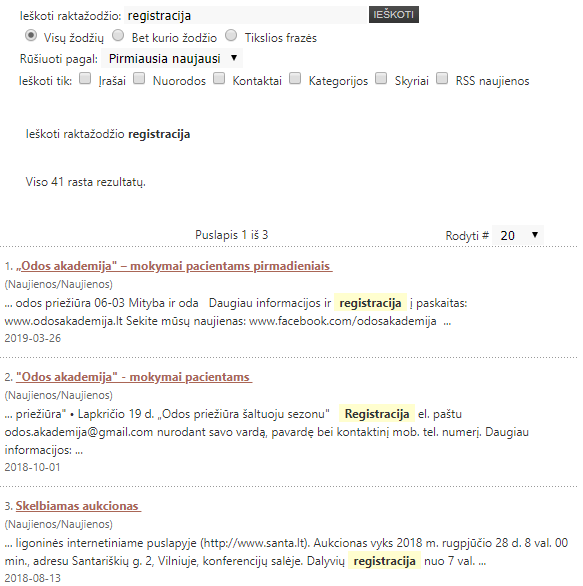
\includegraphics[scale=0.8]{img/BlogaPaieška}
    \caption{Grąžinti rezultatai neteisingai rūšiuojami (\ref{PaieškosLentelėPrad}.3) ir neaktualūs ieškančiam registracijos (\ref{PaieškosLentelėPrad}.7)}
    \label{img:blogapaieška}
\end{figure}

\begin{figure}[H]
    \centering
    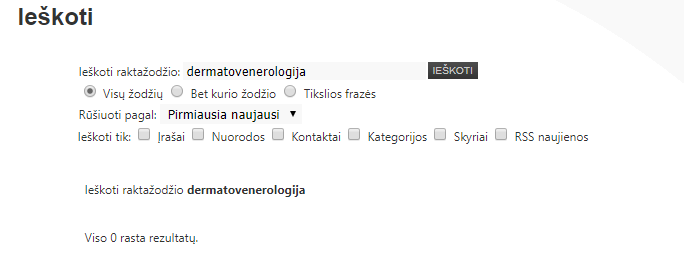
\includegraphics[scale=0.8]{img/TuščiaPaieška}
    \caption{Nėra patarimų kaip pataisyti užklausą (\ref{PaieškosLentelėPrad}.5), nėra šablono sėkmingai paieškai (\ref{PaieškosLentelėPrad}.8) bei pasiektas maksimalus užklausos ilgis (\ref{PaieškosLentelėPrad}.11)}
    \label{img:tuščiapaieška}
\end{figure}

\begin{figure}[H]
    \centering
    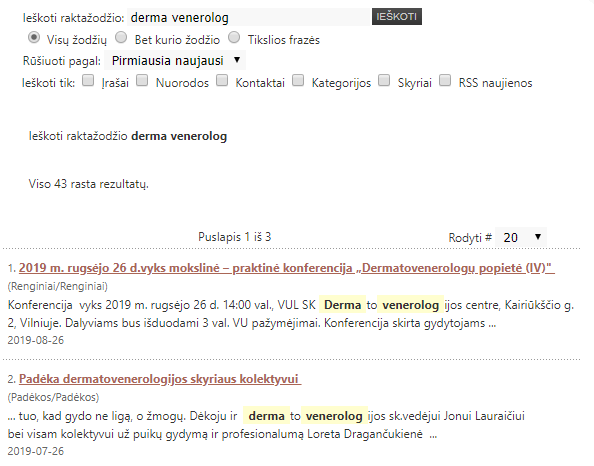
\includegraphics[scale=0.8]{img/ProtingaPaieška}
    \caption{Paieška netikrina panašių galūnių ar rašybos klaidų, taigi reikia gudrauti naudojant žodžių šaknis (\ref{PaieškosLentelėPrad}.19)}
    \label{img:protingapaieška}
\end{figure}

\pagebreak

\subsection{Navigacijos ir informacijos architektūros panaudojamumo analizė}
\begin{center}
\begin{longtable}{ |p{13,5cm}|p{2cm}| } 
 \hline
	Gairė & Ar tenkina? \\ \hline
	1) Yra patogus ir akivaizdus būdas judėti tarp susijusių puslapių ir skyrių ir yra lengva grįžti į pagrindinį puslapį & tenkina \\ \hline
	2) Informacija, kurios naudotojams dažnai prireikia yra lengvai pasiekiama iš daugumos puslapių & tenkina \\ \hline
	3) Navigacijos pasirinkimai išrikiuoti pačiu racionaliausiu arba užduočiai orientuotu būdu & tenkina \\ \hline
	4) Navigacijos sistema plati ir sekli (daug meniu elementų), o ne gili (daug meniu lygių)  & ne (\ref{img:siauranavigacija} pav.) \\ \hline
	5) Paprasta, aiškaus modelio svetainės struktūra be nereikalingų lygių & ne (\ref{img:siauranavigacija} pav.) \\ \hline
	6) Pagrindiniai puslapio skyriai pasiekiami iš bet kurio puslapio ir nėra aklaviečių & tenkina \\ \hline
	7) Navigacijos skirtukai patalpinti puslapio viršuje ir atrodo kaip paspaudžiamos versijos realaus pasaulio skirtukų & ne \\ \hline
	8) Yra svetainės žemėlapis, kuris suteikia svetainės turinio apžvalgą & tenkina \\ \hline
	9) Svetainės žemėlapį galima pasiekti iš bet kurio puslapio & tenkina \\ \hline
	10) Svetainės žemėlapis suteikia glaustą svetainės apžvalgą, o ne pernaudotą navigacijos meniu ar sąrašą kiekvienos temos & ne \\ \hline
	11) Suteikiamas geras navigacijos grįžtamasis ryšys (rodoma, kur randiesi puslapyje) & tenkina \\ \hline
	12) Kategorijų pavadinimai tiksliai apibūdina informaciją viduje & ne (\ref{img:siauranavigacija} pav.) \\ \hline
	13) Nuorodos ir navigacijos pavadinimai susidaro iš raktinių žodžių, kurių naudotojai ieškos bandydami atlikti užduotį & tenkina \\ \hline
	14) Terminologija ir susitarimai (kaip nuorodų spalvos) (maždaug) atitinka bendrą interneto naudojimą & tenkina \\ \hline
	15) Nuorodos atrodo taip pačiai skirtingose svetainės dalyse & tenkina \\ \hline
	16) Navigacijos elementams ir hiperteksto nuorodoms naudojami terminai yra nedviprasmiški ir be žargono & tenkina \\ \hline
	17) Matomi pasikeitimai, kai naudotojas užveda kursorių ant kažko paspaudžiamo (neįskaitant kursoriaus pasikeitimų) & ne \\ \hline
	18) Svarbus turinys pasiekiamas iš daugiau nei vienos nuorodos (naudotojams gali reikėt skirtingų nuorodų pavadinimų) & tenkina \\ \hline
	19) Puslapiai skirti tik navigacijai (pavyzdžiui pradinis puslapis) gali būti peržiūrimi be slinkimo & tenkina \\ \hline
	20) Svetainė leidžia naudotojui kontroliuoti sąveikos greitį ir eiliškumą & tenkina \\ \hline
	21) Visuose puslapiuose yra aiškiai pažymėti išėjimai leidžiantys naudotojui pabėgti iš esamos užduoties be papildomo dialogo & tenkina \\ \hline
	22) Svetainė neišjungia naršyklės „atgal“ mygtuko ir „atgal“ mygtukas visada matomas naršyklės įrankių juostoje & tenkina \\ \hline
	23) Paspaudus „atgal“ mygtuką naudotojas visada gražinamas į puslapį, iš kurio atėjo & tenkina \\ \hline
	24) Jeigu puslapis sukuria naujus langus, jie neklaidina naudotojo (jie dialogo lango dydžio ir lengvai uždaromi) & tenkina \\ \hline
	25) Meniu instrukcijos, nurodymai ir žinutės atsiranda toje pačioje vietoje visuose puslapiuose & tenkina \\ \hline
	%16) Produktų puslapiai turi nuorodas į panašius arba papildomus produktus, kad paskatinti kryžminį pardavimą (angl. cross-selling) &  \\ \hline
	%18) Naudotojai gali rikiuoti ir filtruoti katalogo puslapius (pagal kainą arba populiarumą) & tenkina \\ \hline
	%22) Hipertekso nuorodos, kurios sukelia veiksmus (pavyzdžiui siuntimą) aiškiai skiriasi nuo nuorodų, kurios veda į kitą puslapį &  \\ \hline
	%27) Nuoroda į prekių krepšelį ir atsiskaitymą matomi visuose puslapiuose &  \\ \hline
	\caption{Navigacijos ir informacijos architektūros panaudojamumo gairių vertinimo lentelė pradiniam puslapiui}
	\label{navigacijosirIAlentelėPrad}
\end{longtable}
\end{center}

\ref{navigacijosirIAlentelėPrad} lentelė apima navigacijos ir informacijos architektūros panaudojamumo gaires. Iš 25 gairių dabartinė sistema tenkina 19.
Šioje srityje klaidų nedaug, tačiau kelios iš jų išsiskiria kaip svarbesnės už kitas. Navigacijos sistema yra per siaura pradiniuose lygiuose, todėl į vieną skyrių sueina per daug įvairių elementų. Dėl to kategorijų pavadinimai negali tiksliai apibūdinti informacijos viduje ir sistema turi daugiau lygių, negu galbūt reikėtų (\ref{img:siauranavigacija} pav.).
Kita problema yra vizualinė, užvedus kursorių ant paspaudžiamų elementų šie turėtų pasikeisti, tačiau pirmasis meniu lygis, nuorodos, puslapio kalbos pasirinkimo mygtukai ir paieška nereaguoja į kursorių.

\begin{figure}[H]
    \centering
    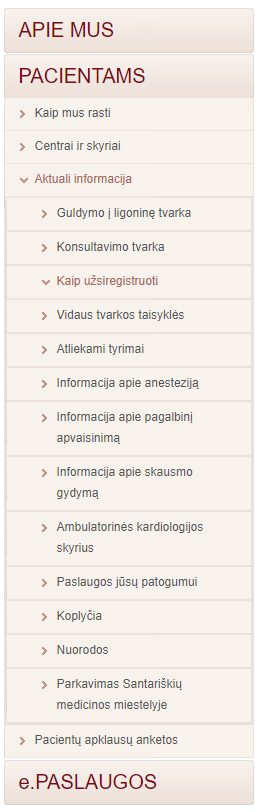
\includegraphics[scale=0.55]{img/SiauraNavigacija}
    \caption{Navigacija turi tik 3 šakas pirmame lygyje (\ref{navigacijosirIAlentelėPrad}.4), dėl to yra nereikalingų lygių (\ref{navigacijosirIAlentelėPrad}.5) ir kategorijos per daug plačios tiksliai apibūdinti informaciją viduje (\ref{navigacijosirIAlentelėPrad}.12)}
    \label{img:siauranavigacija}
\end{figure}

\subsection{Bendro panaudojamumo analizė}

\begin{center}
\begin{tabular}{ | p{4cm} | p{0,5cm} | p{11cm} | } 
 \hline
	Euristika & DS & Komentaras \\ \hline
	1) Sistemos būsenos matomumas & 2 & Paspaudus mygtuką „ieškoti“ rodomas tuščias puslapis iki paieškos rezultatų gavimo. Paieška užtrunka apie 3 sekundes, taigi galėtų būti tekstas, animacija ar progreso juosta pranešanti, kad vyksta paieška. Užvedus kursorių ant paspaudžiamų elementų kaip nuorodų ir tam tikrų elementų, šie nepasikeičia, taigi vartotojui sunkiau juos pastebėti. \\ \hline
	2) Atitikimas realiam pasauliui  & 2 & Daugumai vartotojų aktuali registracija pas gydytoją, taigi ji turėtų būti dar lengviau surandama naršant arba ieškant (\ref{img:blogapaieška}, \ref{img:RegistracijaPagrindinis} ir \ref{img:registracija} pav.). \\ \hline
	3) Naudotojo valdomas dialogas & 1 & Dalis puslapių nerodo nukeliauto kelio, kai šie randami per paiešką (\ref{img:atvaizdavimoklaida} pav.). \\ \hline
	4) Darna ir standartai & 1 & Kai kuriuose puslapiuose pranyksta navigacijos elementai (\ref{img:atvaizdavimoklaida} pav.) \\ \hline
	5) Klaidų prevencija & 2 & Netinkami numatytieji nustatymai lemia, kad naudotojai dažnai atlieka netinkamą paiešką (\ref{img:blogapaieška}, \ref{img:tuščiapaieška} ir \ref{img:protingapaieška} pav.). Nėra patarimų kaip naudotis paieškos sistema. Vedant užklausą nepasiūlomi paieškos variantai. \\ \hline
	6) Atpažinimas geriau nei atsiminimas & 2 & Navigacija nerodo gilesnių lygių, kol neatidaromas to lygio puslapis, taigi reikia žinoti, kurioje kategorije ieškomas elementas (\ref{img:siauranavigacija} pav.). Trūksta vaizdų, kurie asocijuojasi su mygtukais. Nėra pagalbos naudotis tinklapiu. \\ \hline
	7) Naudojimo lankstumas ir našumas & 2 & Nerodomi susiję puslapiai. Negalima nueiti į giliausią kategorijos lygį vienu paspaudimu, reikia eiti per tėvinius elementus (\ref{img:siauranavigacija} pav.). \\ \hline
	8) Estetiškas ir minimalistinis dizainas & 2 & Pertekliniai paspaudimai bandant naviguoti per kategorijas (\ref{img:siauranavigacija} pav.). \\ \hline
	9) Remti klaidų atpažinimą, jų priežasčių nustatymą ir taisymą & 0 &  \\ \hline
	10) Parama ir dokumentacija & 2 & Nėra informacijos ar pavyzdžių kaip naudoti sudėtingas paieškos funkcijas (\ref{img:blogapaieška} pav.). \\ \hline
\end{tabular}
\captionof{table}{Euristinio vertinimo lentelė}
\label{EuristikųLentelėPrad}
\end{center}

%Iš bendro panaudojamumo vertinimo rasta dar panaudojamumo problemų. 

\begin{figure}[H]
    \centering
    
\includegraphics[scale=0.6]{img/RegistracijaPagrindinis}
    \caption{Registracija pas gydytoją yra prastai pastebimoje vietoje (\ref{EuristikųLentelėPrad}.2)}
    \label{img:RegistracijaPagrindinis}
\end{figure}

\begin{figure}[H]
    \centering
    
\includegraphics[scale=0.8]{img/RegistracijosAklavietė}
    \caption{Registracijos aklavietė (\ref{EuristikųLentelėPrad}.2)}
    \label{img:registracija}
\end{figure}

\begin{figure}[H]
    \centering
    
\includegraphics[scale=0.55]{img/AtvaizdavimoKlaida}
    \caption{Pranykusi didžioji dalis navigacijos ir vizualinė klaida paieškos lange}
    \label{img:atvaizdavimoklaida}
\end{figure}

%Medžiagos darbo tema dėstymo skyriuose pateikiamos nagrinėjamos temos detalės:
%pradinė medžiaga, jos analizės ir apdorojimo metodai, sprendimų įgyvendinimas,
%gautų rezultatų apibendrinimas. Šios dalies turinys labai priklauso nuo darbo
%temos. Skyriai gali turėti poskyrius ir smulkesnes sudėtines dalis, kaip
%punktus ir papunkčius.

%Medžiaga turi būti dėstoma aiškiai, pateikiant argumentus. Tekstas dėstomas
%trečiuoju asmeniu, t.y. rašoma ne „aš manau“, bet „autorius mano“, „autoriaus
%nuomone“. Reikėtų vengti informacijos nesuteikiančių frazių, pvz., „...kaip jau
%buvo minėta...“, „...kaip visiems žinoma...“ ir pan., vengti grožinės literatūros
%ar publicistinio stiliaus, gausių metaforų ar panašių meninės išraiškos
%priemonių.



\section{Galutinio sprendimo maketas}
%Kuriant sprendimo maketus remiamasi jau egzistuojančiais ligoninių puslapiais, kurie atitinka prisitaikančio dizaino (angl. responsive design) principus. Prisitaikantis dizainas leidžia turėti vieną puslapį, kuris prisitaiko prie įvarių ekrano formų ir dydžių\cite{RWDEn}. Pavyzdiniai puslapiai parinkti iš didmiesčių ligoninių, Vilniaus, Kauno ir Niujorko. Autoriaus subjektyvia nuomone Kauno ligonės puslapis yra ypač geras pavyzdys. Sumuštinio meniu, registracijos mygtukas ir paieška yra geriausiai matomoje vietoje, naudojami dideli mygtukai su aiškiais užrašais bei kontrastingos spalvos, taigi net žmonėms su prastu regėjimu turėtų būti patogu naudotis (\ref{img:kaunomobile} pav.).
Šiame skyriuje analizuojami autoriaus sukurti maketai skirti išspręsti tinklapio panaudojamumo problemas pastebėtas praėjusiame skyriuje. Maketams kurti galima naudoti vieną iš daugelio įrankių: Adobe XD, Axure RP, Balsamique, Moqups, Justinmind ir kiti. Šiuo atveju naudojamas Moqups vartotojo sąsajos maketų kūrimo įrankis.

Per panaudojamumo analizę aptikta, kad tinklapis daugiau tenkina, nei netenkina gaires. Autoriaus nuomone puslapių projektavimas yra iteracinis procesas, taigi dauguma esamojo tinklapio elementų palikti koki buvo. Pakeitimai atlikti tose vietose, kur pastebėti trūkumai. Maketuose prasmingi pakeitimai pažymėti raudonai.

\begin{figure}[H]
    \centering
    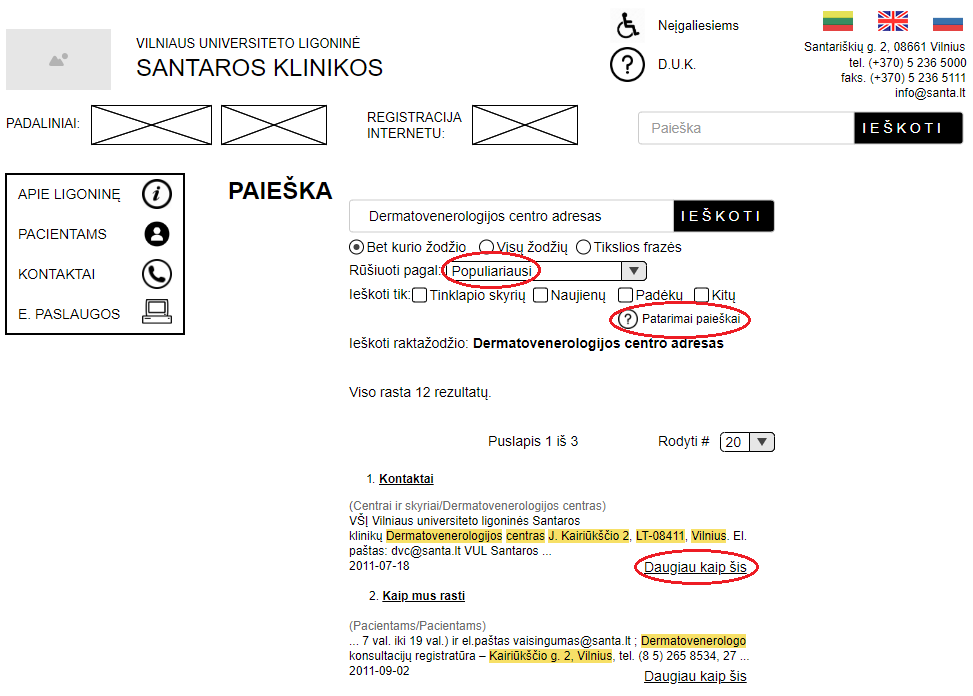
\includegraphics[scale=0.65]{img/PaieškosPrototipas}
    \caption{Paieškos sistemos maketas su sistemos pataisymais}
    \label{img:PaieškosPrototipas}
\end{figure}

\ref{img:PaieškosPrototipas} paveikslėlyje pavaizduotas paieškos sistemos maketas. Šiame makete pakeistas numatytasis paieškos rūšiavimo būdas iš rūšiavimo pagal naujumą į rūšiavimą pagal populiarumą (\ref{PaieškosLentelėPrad}.3, \ref{EuristikųLentelėPrad}.2 ir \ref{EuristikųLentelėPrad}.5 defektas). Maketas turi pagalbos laukelį, kuris duoda patarimų kaip naudotis paieška (\ref{PaieškosLentelėPrad}.5, \ref{PaieškosLentelėPrad}.8, \ref{EuristikųLentelėPrad}.5  ir \ref{EuristikųLentelėPrad}.10 defektas). Defektas \ref{PaieškosLentelėPrad}.7 kyla iš paieškos sistemos suprogramavimo, taigi šis maketas negali jo pataisyti, tačiau jau minėtas rūšiavimo pakeitimas turėtų bent dalinai mitiguoti problemą, nes naudingi rezultatai bus iškelti į viršų, kai tokių yra. Defektas \ref{PaieškosLentelėPrad}.11 vėlgi susijęs su paieškos implementacija. Atlikus šiuos paieškos sistemos pakeitimus turėtų palengvėti naudojimasis paieška, kas skatina paieškos strategiją ieškant informacijos (\ref{PaieškosLentelėPrad}.16 defektas). Defektas \ref{PaieškosLentelėPrad}.19 irgi priklauso nuo paieškos kodo. Makete po kiekvienu paieškos rezultatu pridėtas mygtukas „Daugiau kaip šis“, kuris leistų atlikti panašių elementų paiešką (\ref{PaieškosLentelėPrad}.20 defektas).


\begin{figure}[H]
    \centering
    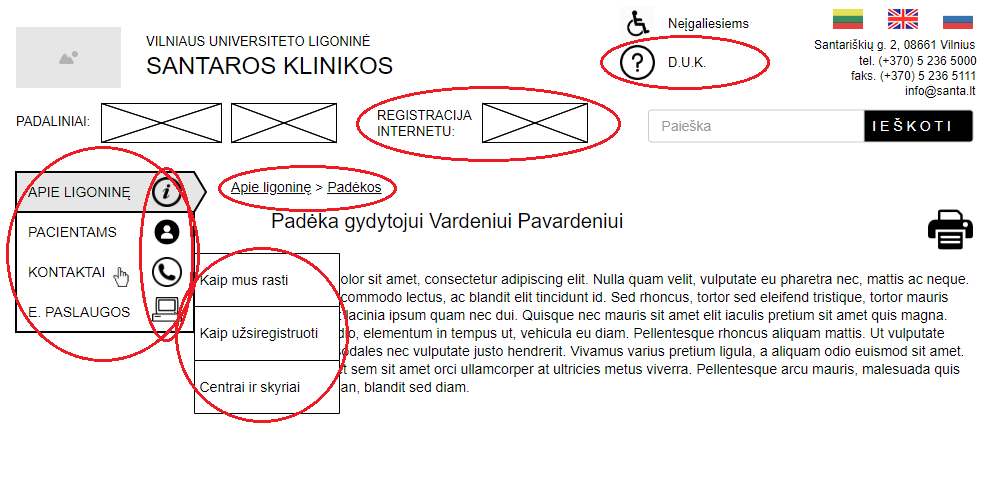
\includegraphics[scale=0.65]{img/NavigacijosPrototipas}
    \caption{Navigacijos sistemos maketas su sistemos pataisymais}
    \label{img:NavigacijosPrototipas}
\end{figure}

\ref{img:NavigacijosPrototipas} paveikslėlyje pavaizduotas navigacijos sistemos maketas. Makete pirmas navigacijos lygis praplatintas viena kategorija, kas leidžia visus elementus logiškai sudėti į antrą lygį (\ref{NavigacijosirIALentelėPrad}.4, \ref{NavigacijosirIALentelėPrad}.5 ir \ref{EuristikųLentelėPrad}.2 defektas). Viršutinėje puslapio dalyje pridėtas mygtukas elektroninei registracijai pas gydytoją (\ref{EuristikųLentelėPrad}.2 defektas). Per navigacijos sistemą visada matoma aktyvi kategorija (kurioje naudotojas dabar naršo) ir nukeliautas kelias, kuris turi nuorodas į tėvinius lygius (\ref{EuristikųLentelėPrad}.3 ir \ref{EuristikųLentelėPrad}.4 defektas). Užvedus pelę ant navigacijos dabar parodomi žemiau esantys lygiai (\ref{EuristikųLentelėPrad}.6, \ref{EuristikųLentelėPrad}.7 ir \ref{EuristikųLentelėPrad}.8 defektas). Pridėti paveiksliukai prie kategorijų, leidžiantys naudotojui lengviau atpažinti kategorijas (\ref{EuristikųLentelėPrad}.6 defektas). Pridėtas D.U.K. (Dažnai užduodamų klausimų) mygtukas, kuris nuvestų į pagalbinį puslapį (\ref{EuristikųLentelėPrad}.6 defektas).


\section{Reikalavimai galutinio sprendimo įgyvendinimui}

Norint sukurti galutinį sprendimą liko išspręsti dar keletą problemų, šiame skyriuje nagrinėjamos šios problemos. 

%\section{Technologijos galutinio sprendimo įgyvendinimui}

\sectionnonum{Rezultatai ir išvados}

%Rezultatų ir išvadų dalyje turi būti aiškiai išdėstomi pagrindiniai darbo
%rezultatai (kažkas išanalizuota, kažkas sukurta, kažkas įdiegta) ir pateikiamos
%išvados (daromi nagrinėtų problemų sprendimo metodų palyginimai, teikiamos
%rekomendacijos, akcentuojamos naujovės).


%% PAKEISTAS PAVADINIMAS Į 'Šaltiniai'
\printbibliography[heading=bibintoc, title=Šaltiniai]  % Šaltinių sąraše nurodoma panaudota
% literatūra, kitokie šaltiniai. Abėcėlės tvarka išdėstomi darbe panaudotų
% (cituotų, perfrazuotų ar bent paminėtų) mokslo leidinių, kitokių publikacijų
% bibliografiniai aprašai.  Šaltinių sąrašas spausdinamas iš naujo puslapio.
% Aprašai pateikiami netransliteruoti. Šaltinių sąraše negali būti tokių
% šaltinių, kurie nebuvo paminėti tekste.

% \sectionnonum{Sąvokų apibrėžimai}
%\sectionnonum{Santrumpos}
%Sąvokų apibrėžimai ir santrumpų sąrašas sudaromas tada, kai darbo tekste
%vartojami specialūs paaiškinimo reikalaujantys terminai ir rečiau sutinkamos
%santrumpos.

%\appendix  % Priedai
% Prieduose gali būti pateikiama pagalbinė, ypač darbo autoriaus savarankiškai
% parengta, medžiaga. Savarankiški priedai gali būti pateikiami ir
% kompaktiniame diske. Priedai taip pat numeruojami ir vadinami. Darbo tekstas
% su priedais susiejamas nuorodomis.






%\section{Eksperimentinio palyginimo rezultatai}
% tablesgenerator.com - converts calculators (e.g. excel) tables to LaTeX
%\begin{table}[H]\footnotesize
%  \centering
%  \caption{Lentelės pavyzdys}
%  {\begin{tabular}{|l|c|c|} \hline
%    Algoritmas & $\bar{x}$ & $\sigma^{2}$ \\
%    \hline
%    Algoritmas A  & 1.6335    & 0.5584       \\
%    Algoritmas B  & 1.7395    & 0.5647       \\
%    \hline
%  \end{tabular}}
%  \label{tab:table example}
%\end{table}

\end{document}
